\documentclass[border=4pt,12pt]{standalone}
% House style for redrawn exam diagrams (diagram-v4: 0.4pt lines, filled -latex arrows, fine dashes; stipple and hatching drawn as real dots/lines (no PDF/SVG patterns, so they render in every browser and at any scale); transparent background). Every figure \input's this.
\usepackage{amsmath,amssymb}
\usepackage{txfonts}
\usepackage{pdfrender,xcolor}
% \halo{text}: label on shading. The shading stops just around each letter's outline (a thin knock-out that follows the
% glyphs, like the papers' typesetting), never a box. Owner: "I don't want a box around the text".
\newcommand{\halo}[1]{\leavevmode\rlap{\pdfrender{TextRenderingMode=2,LineWidth=2.2pt,LineJoinStyle=1,StrokeColor=white,FillColor=white}#1}#1}
\usepackage{tikz,pgfplots}
\pgfplotsset{compat=1.18}
\usetikzlibrary{arrows.meta,calc,angles,quotes,patterns,patterns.meta,intersections,positioning,decorations.markings,shapes.geometric}
% Stipple and hatching are drawn as actual dots / lines clipped to the region (path picture), NOT as pattern fills:
% SVG <pattern> fills vanish or blur when browsers scale the image, so the owner could not see the shading.
% Each dot is a 0.72pt square (keeps SVGs small; reads as a dot at print size). Dots sit on one global staggered grid, so neighbouring regions line up.
\makeatletter
\newdimen\ex@x \newdimen\ex@y \newdimen\ex@xa \newdimen\ex@ya \newdimen\ex@xb \newdimen\ex@yb \newcount\ex@row
\def\exam@stipplecolor{black!75}\def\exam@dotr{0.42pt}\def\exam@dotgap{2.5}
\def\ex@rowdots{\ifdim\ex@x<\ex@xb \pgfpathrectangle{\pgfqpoint{\dimexpr\ex@x-0.36pt\relax}{\dimexpr\ex@y-0.36pt\relax}}{\pgfqpoint{0.72pt}{0.72pt}}\advance\ex@x by \exam@dotgap pt\relax\expandafter\ex@rowdots\fi}
\def\exam@stipple{%
  \pgftransformreset% dots are sized in real points even inside scaled pictures
  \pgfpointanchor{path picture bounding box}{south west}\ex@xa=\pgf@x \ex@ya=\pgf@y
  \pgfpointanchor{path picture bounding box}{north east}\ex@xb=\pgf@x \ex@yb=\pgf@y
  \pgfsetfillcolor{\exam@stipplecolor}\pgfmathsetmacro\ex@h{\exam@dotgap/2}%
  \pgfmathtruncatemacro\ex@r{floor(\ex@ya/\ex@h)-1}\ex@row=\ex@r\relax
  \ex@y=\ex@r\dimexpr\ex@h pt\relax
  \loop\ifdim\ex@y<\ex@yb
    \pgfmathtruncatemacro\ex@c{floor(\ex@xa/\exam@dotgap)-1}\ex@x=\ex@c\dimexpr\exam@dotgap pt\relax
    \ifodd\ex@row \advance\ex@x by \ex@h pt\fi
    \ex@rowdots
    \advance\ex@y by \ex@h pt \advance\ex@row by 1
    \ifnum\numexpr\ex@row-(\ex@row/4)*4\relax=0 \pgfusepath{fill}\fi% flush every 4 rows: bounded TeX memory, few clip copies in the SVG
  \repeat\pgfusepath{fill}}
\newdimen\ex@d
\def\exam@hatch#1{% #1 = 1 for /, -1 for \ ; lines 45 degrees, 3pt apart
  \pgftransformreset
  \pgfpointanchor{path picture bounding box}{south west}\ex@xa=\pgf@x \ex@ya=\pgf@y
  \pgfpointanchor{path picture bounding box}{north east}\ex@xb=\pgf@x \ex@yb=\pgf@y
  \ex@d=\dimexpr\ex@yb-\ex@ya\relax \ex@x=\dimexpr\ex@xa-\ex@d\relax
  \loop\ifdim\ex@x<\ex@xb
    \ifnum#1>0 \pgfpathmoveto{\pgfqpoint{\ex@x}{\ex@ya}}\pgfpathlineto{\pgfqpoint{\dimexpr\ex@x+\ex@d\relax}{\ex@yb}}%
    \else \pgfpathmoveto{\pgfqpoint{\ex@x}{\ex@yb}}\pgfpathlineto{\pgfqpoint{\dimexpr\ex@x+\ex@d\relax}{\ex@ya}}\fi
    \advance\ex@x by 4.24pt
  \repeat
  \pgfsetlinewidth{0.4pt}\pgfsetstrokecolor{black}\pgfusepath{stroke}}
\def\examstipple{\exam@stipple}\def\examhatch{\exam@hatch}\def\examsetstipplecolor#1{\def\exam@stipplecolor{#1}}\def\examsetdotgap#1{\def\exam@dotgap{#1}}
\makeatother
% (legacy pattern kept for old files)
% staggered stipple like the NESA papers' dotted shading
\pgfdeclarepatternformonly{exam stipple}{\pgfpointorigin}{\pgfqpoint{2.2pt}{2.2pt}}{\pgfqpoint{2.2pt}{2.2pt}}{%
  \pgfpathcircle{\pgfqpoint{0.55pt}{0.55pt}}{0.42pt}\pgfpathcircle{\pgfqpoint{1.65pt}{1.65pt}}{0.42pt}\pgfusepath{fill}}
\tikzset{
  every picture/.style={line width=0.6pt, >={Latex[length=2mm,width=1.3mm]}},
  curve/.style={line width=0.6pt},
  open arrow/.style={-{Latex[length=2mm,width=1.3mm]}},  % owner: filled -latex heads everywhere, no open chevrons
  aux/.style={dash pattern=on 2pt off 1.5pt, line width=0.6pt},
  shade/.code={\def\exA{#1}\def\exB{none}\ifx\exA\exB\else\pgfkeysalso{fill=black!18}\fi},
  shade/.default=on,
  shade dots/.style={fill=none, path picture={\examstipple}},
  stipple color/.code={\examsetstipplecolor{#1}},
  stipple gap/.code={\examsetdotgap{#1}},
  shade dense dots/.style={fill=none, stipple gap=1.6, path picture={\examstipple}},
  shade hatch/.style={fill=none, path picture={\examhatch{1}}},
  shade hatch reverse/.style={fill=none, path picture={\examhatch{-1}}},
  shade solid/.style={fill=black},
  pt/.style={circle, fill, inner sep=1.1pt},
  open pt/.style={circle, draw, fill=white, inner sep=1.1pt},
}
\pgfplotsset{
  exam axes/.style={axis lines=middle, axis line style={->}, xlabel={$x$}, ylabel={$y$},
    xlabel style={anchor=west}, ylabel style={anchor=south}, tick label style={font=\small},
    every axis plot/.append style={line width=0.6pt, black}, samples=200, clip=false,
    enlargelimits=false, axis on top},
}

\begin{document}
% crop pixels, y down; curve traced from the crop
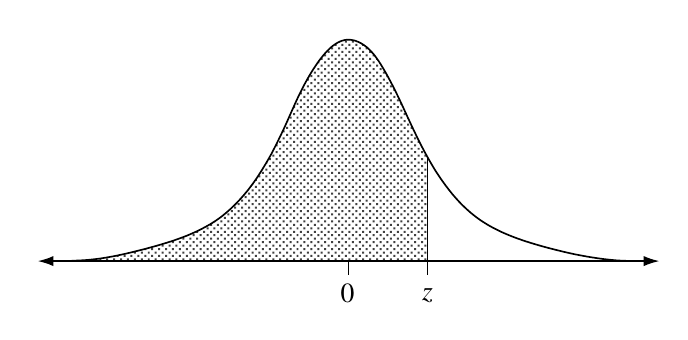
\begin{tikzpicture}[x=0.0127cm, y=-0.0127cm]
  \begin{scope}
    \clip (0,0) rectangle (400,233.5);
    \path[shade dots] plot[smooth] coordinates {(44,233.2) (58.03,232.5) (71.97,231) (86.28,228.6) (101.1,225.4) (116,221.7) (131.3,217.5) (145.5,213.1) (158.9,208.2) (171.3,202.7) (182.6,196.6) (192.7,189.9) (202.3,181.9) (211.4,172.9) (220.2,162.7) (228.4,151.6) (236,139.7) (243.4,127) (250.2,113.7) (256.9,99.73) (263.6,84.73) (270.1,70.36) (276.7,57.11) (283.6,44.97) (290.9,33.92) (298.2,24.83) (305,18.35) (311.1,14.42) (316.6,12.46) (321.6,12) (327.3,12.94) (333.3,15.49) (339.5,19.74) (345.8,26.17) (352.2,35.07) (359.4,47.22) (366.4,60.49) (373.2,74.5) (380.1,89.5) (387,104.2) (393.8,118) (401,131.3) (408.4,143.8) (416.3,155.4) (424.7,166.3) (433.4,176) (442.7,184.7) (452.4,192.2) (463,198.8) (474.5,204.6) (487.3,209.9) (501,214.6) (515.5,218.9) (530.5,222.8) (545.5,226.3) (560.3,229.1) (574.8,231.3) (589.4,232.8) (603.7,233.4) (618,233.3)} -- cycle;
  \end{scope}
  \draw[<->] (10,233.5) -- (632,233.5);
  \draw plot[smooth] coordinates {(44,233.2) (58.03,232.5) (71.97,231) (86.28,228.6) (101.1,225.4) (116,221.7) (131.3,217.5) (145.5,213.1) (158.9,208.2) (171.3,202.7) (182.6,196.6) (192.7,189.9) (202.3,181.9) (211.4,172.9) (220.2,162.7) (228.4,151.6) (236,139.7) (243.4,127) (250.2,113.7) (256.9,99.73) (263.6,84.73) (270.1,70.36) (276.7,57.11) (283.6,44.97) (290.9,33.92) (298.2,24.83) (305,18.35) (311.1,14.42) (316.6,12.46) (321.6,12) (327.3,12.94) (333.3,15.49) (339.5,19.74) (345.8,26.17) (352.2,35.07) (359.4,47.22) (366.4,60.49) (373.2,74.5) (380.1,89.5) (387,104.2) (393.8,118) (401,131.3) (408.4,143.8) (416.3,155.4) (424.7,166.3) (433.4,176) (442.7,184.7) (452.4,192.2) (463,198.8) (474.5,204.6) (487.3,209.9) (501,214.6) (515.5,218.9) (530.5,222.8) (545.5,226.3) (560.3,229.1) (574.8,231.3) (589.4,232.8) (603.7,233.4) (618,233.3)};
  \draw (400,128.5) -- (400,247);
  \draw (321,233.5) -- (321,247);
  \node at (320,265.5) {$0$};
  \node at (400,268) {$z$};
\end{tikzpicture}
\end{document}
